% htts://pxl-digital.pxl.be/page/studentenreis-2020-berlijn2

Als internationaliseringsonderdeel was er de mogelijkheid om op studiereis te gaan met medestudenten. Ik heb deze kans gegrepen en heb gekozen voor de studiereis naar Berlijn. Er waren verschillende reizen, één naar Amsterdam en twee naar Berlijn. Die naar Amsterdam heb ik niet gekozen omdat ik al vaker naar die stad ben gegaan en Cisco, wat mij niet echt aanspreekt, was daar de hoofdzaak. Dus er bleven nog twee reizen naar Berlijn over, en ik verkoos het om naar de universiteit te gaan dan deel te nemen aan de makathon.

De reis begon natuurlijk met een lange busrit, hier leerde we elkaar al wat beter kennen en wisten we wie er allemaal mee ging. Eenmaal aangekomen konden we inchecken in de kamer van het hotel en hadden we de rest van de avond nog vrij om Berlijn te gaan verkennen of om uit te rusten voor de drukke dagen die we tegemoet stonden.

De eerste echte dag in Berlijn werden we opgesplitst in twee groepen om afwisselend de geplande activiteiten uit te voeren. Zo vertrok de ene groep naar de Stasi\hyp{}gevangenis Hohensch\"onhausen en de andere naar de Tempelhof luchthaven. Na de middag wisselde de groepen van activiteit. In de gevangenis kregen we een rondleiding van een ex\hyp{}gevangene, dit was een voor\hyp{} en een nadeel. Zijn Engels was niet zo goed waardoor hij in het begin moeilijk te verstaan was, maar nadien kon hij zeer mooi zijn ervaringen en gevoelens delen met ons wat het zeer interessant maakte. Hij had een zeer fascinerende houding tegenover de gevangenis en de bewakers van toen.

Daarna kregen we een rondleiding in de luchthaven, wat vroeger een van de grootste gebouwen van Europa was. Hier hebben we natuurlijk veel moeten wandelen om het volledige gebouw te zien, maar dat was zeker de moeite. De luchthaven toen wij het bezochten was volledig leeg en verlaten op een paar ruimtes na. Dankzij de goede uitleg en aanvullende attributen kregen we toch een goed idee over hoe de luchthaven functioneerde in zijn hoogtepunt en waarom dat hij nog zo goed intact is gebleven geduurde de oorlog. En ook wat de zijn huidige functie is en wat er in de toekomst nog mee zou kunnen gebeuren.

De volgende dag was er een toeristische rondleiding gepland in Berlijn. Zo reden we eerst met de bus door Berlijn en gaf een gids uitleg over monumenten en straten waar we langs of door reden. Na deze busrit gingen we te voet verder met de gids. Zo bezochten we monumenten als de Berlijnse Muur, Checkpoint Charlie, Potsdamer Platz, de Berliner Dom, het Holocause monument en nog veel meer. De gids gaf een goede uitleg over het verleden van deze monumenten maar ook de huidige betekenis en waarde ervan. Normaal gezien ben ik geen fan van een rondleiding met een gids, maar hier was ik zeer aangenaam van verrast omdat we ook veel hebben kunnen zien op een korte tijd met een nuttige uitleg.

\begin{figure}[!h]
  \centering
  \begin{subfigure}[h]{0.48\textwidth}
    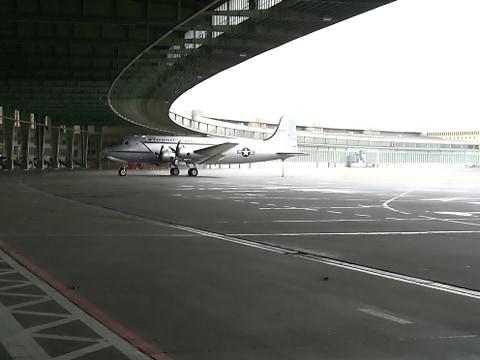
\includegraphics[width=\linewidth]{berlijn/tempelhof.jpg}
    \caption{Tempelhof luchthaven}
  \end{subfigure}
  \begin{subfigure}[h]{0.48\textwidth}
    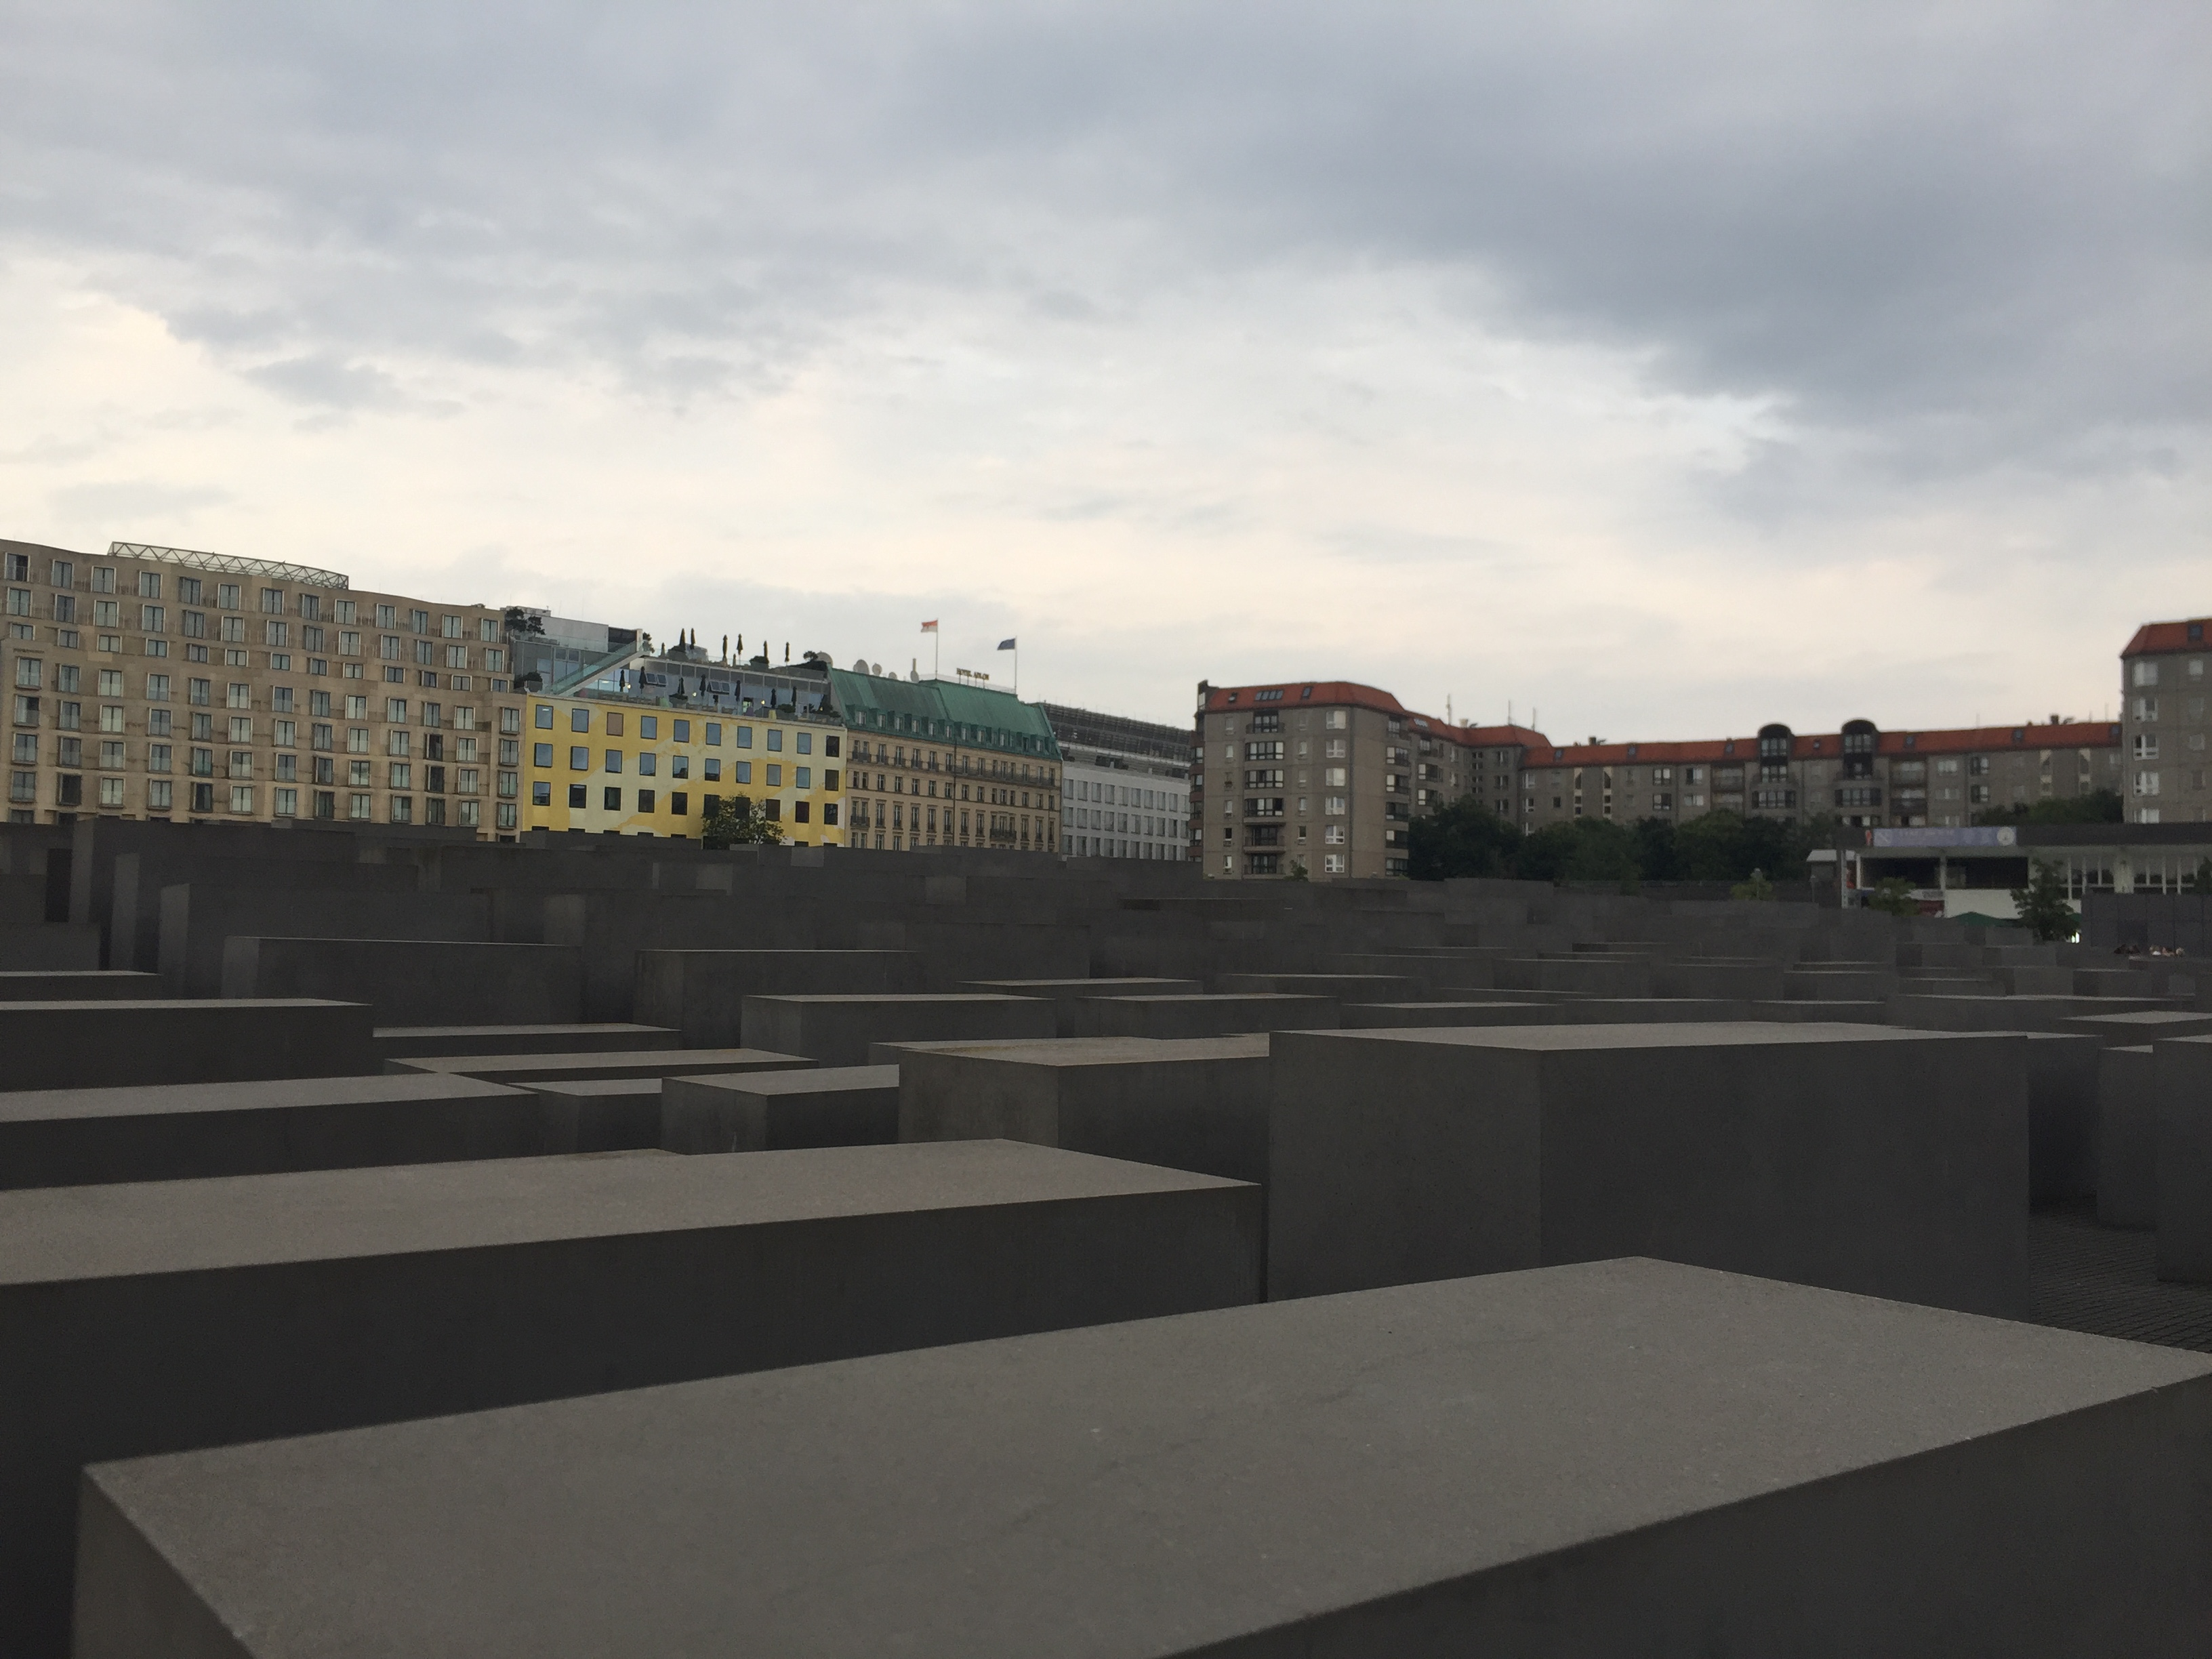
\includegraphics[width=\linewidth]{berlijn/holocaust_monument.jpg}
    \caption{Holocaust monument}
  \end{subfigure}
\end{figure}

De laatste dag in Berlijn zouden we normaal naar de Technische Universit\"at Berlin gaan en daar een seminarie volgen rond Future Security Lab, maar dit is niet doorgegaan om een voor ons onbekende reden. Na de middag kregen we daar ook een seminarie dat nog niet bekend was, maar deze hebben we uiteraard ook niet kunnen volgen. Omdat onze begeleiders deze late annulering niet hadden voorzien, mochten we deze dag zelf inplannen. Ik ben dan met een paar vrienden Berlijn nog wat verder gaan verkennen en op het gemak wat genieten en uitrusten van de vermoeide afgelopen dagen. Na een korte nacht konden vlug uitchecken van het hotel en ontbijten voor we de bus weer opstapte richting Hasselt.

De studiereis was zeker geslaagd voor mij, alleen vond ik het jammer dat we niet naar de universiteit zijn kunnen gaan. Ik heb mijn medestudenten zeker beter leren kennen en daar nieuwe vrienden gemaakt, wat ik niet had verwacht voor ik vertrok op de reis. Ik ga wel vaker op reis, dus ik wist wel waar ik mij aan moest verwachten, maar om dit met een school te doen is wel nog een andere ervaring.

Op de onvoorziene omstandigheden na, zou ik de reis zeker opnieuw doen en aanraden voor andere studenten. Het enige waar ik niet naar zou uitkijken zijn de busritten, maar die horen er natuurlijk wel bij. Het was zeker wel een vermoeiende reis, korte nachten en lange dagen, zo leer je elkaar wel veel beter kennen op een korte periode.

Ik heb deze opdracht opgenomen in mijn portfolio omdat deze studiereis toch wel een grote indruk heeft nagelaten en het een groot deel uitmaakte van mijn derde en belangrijkste jaar op Hogeschool PXL. Ook omdat op gebied van mijn medestudenten leren kennen, dit toch een van de meest impactvolle elementen is en het plezier maken met elkaar.

\begin{figure}[!h]
  \centering
  \begin{subfigure}[h]{0.48\textwidth}
    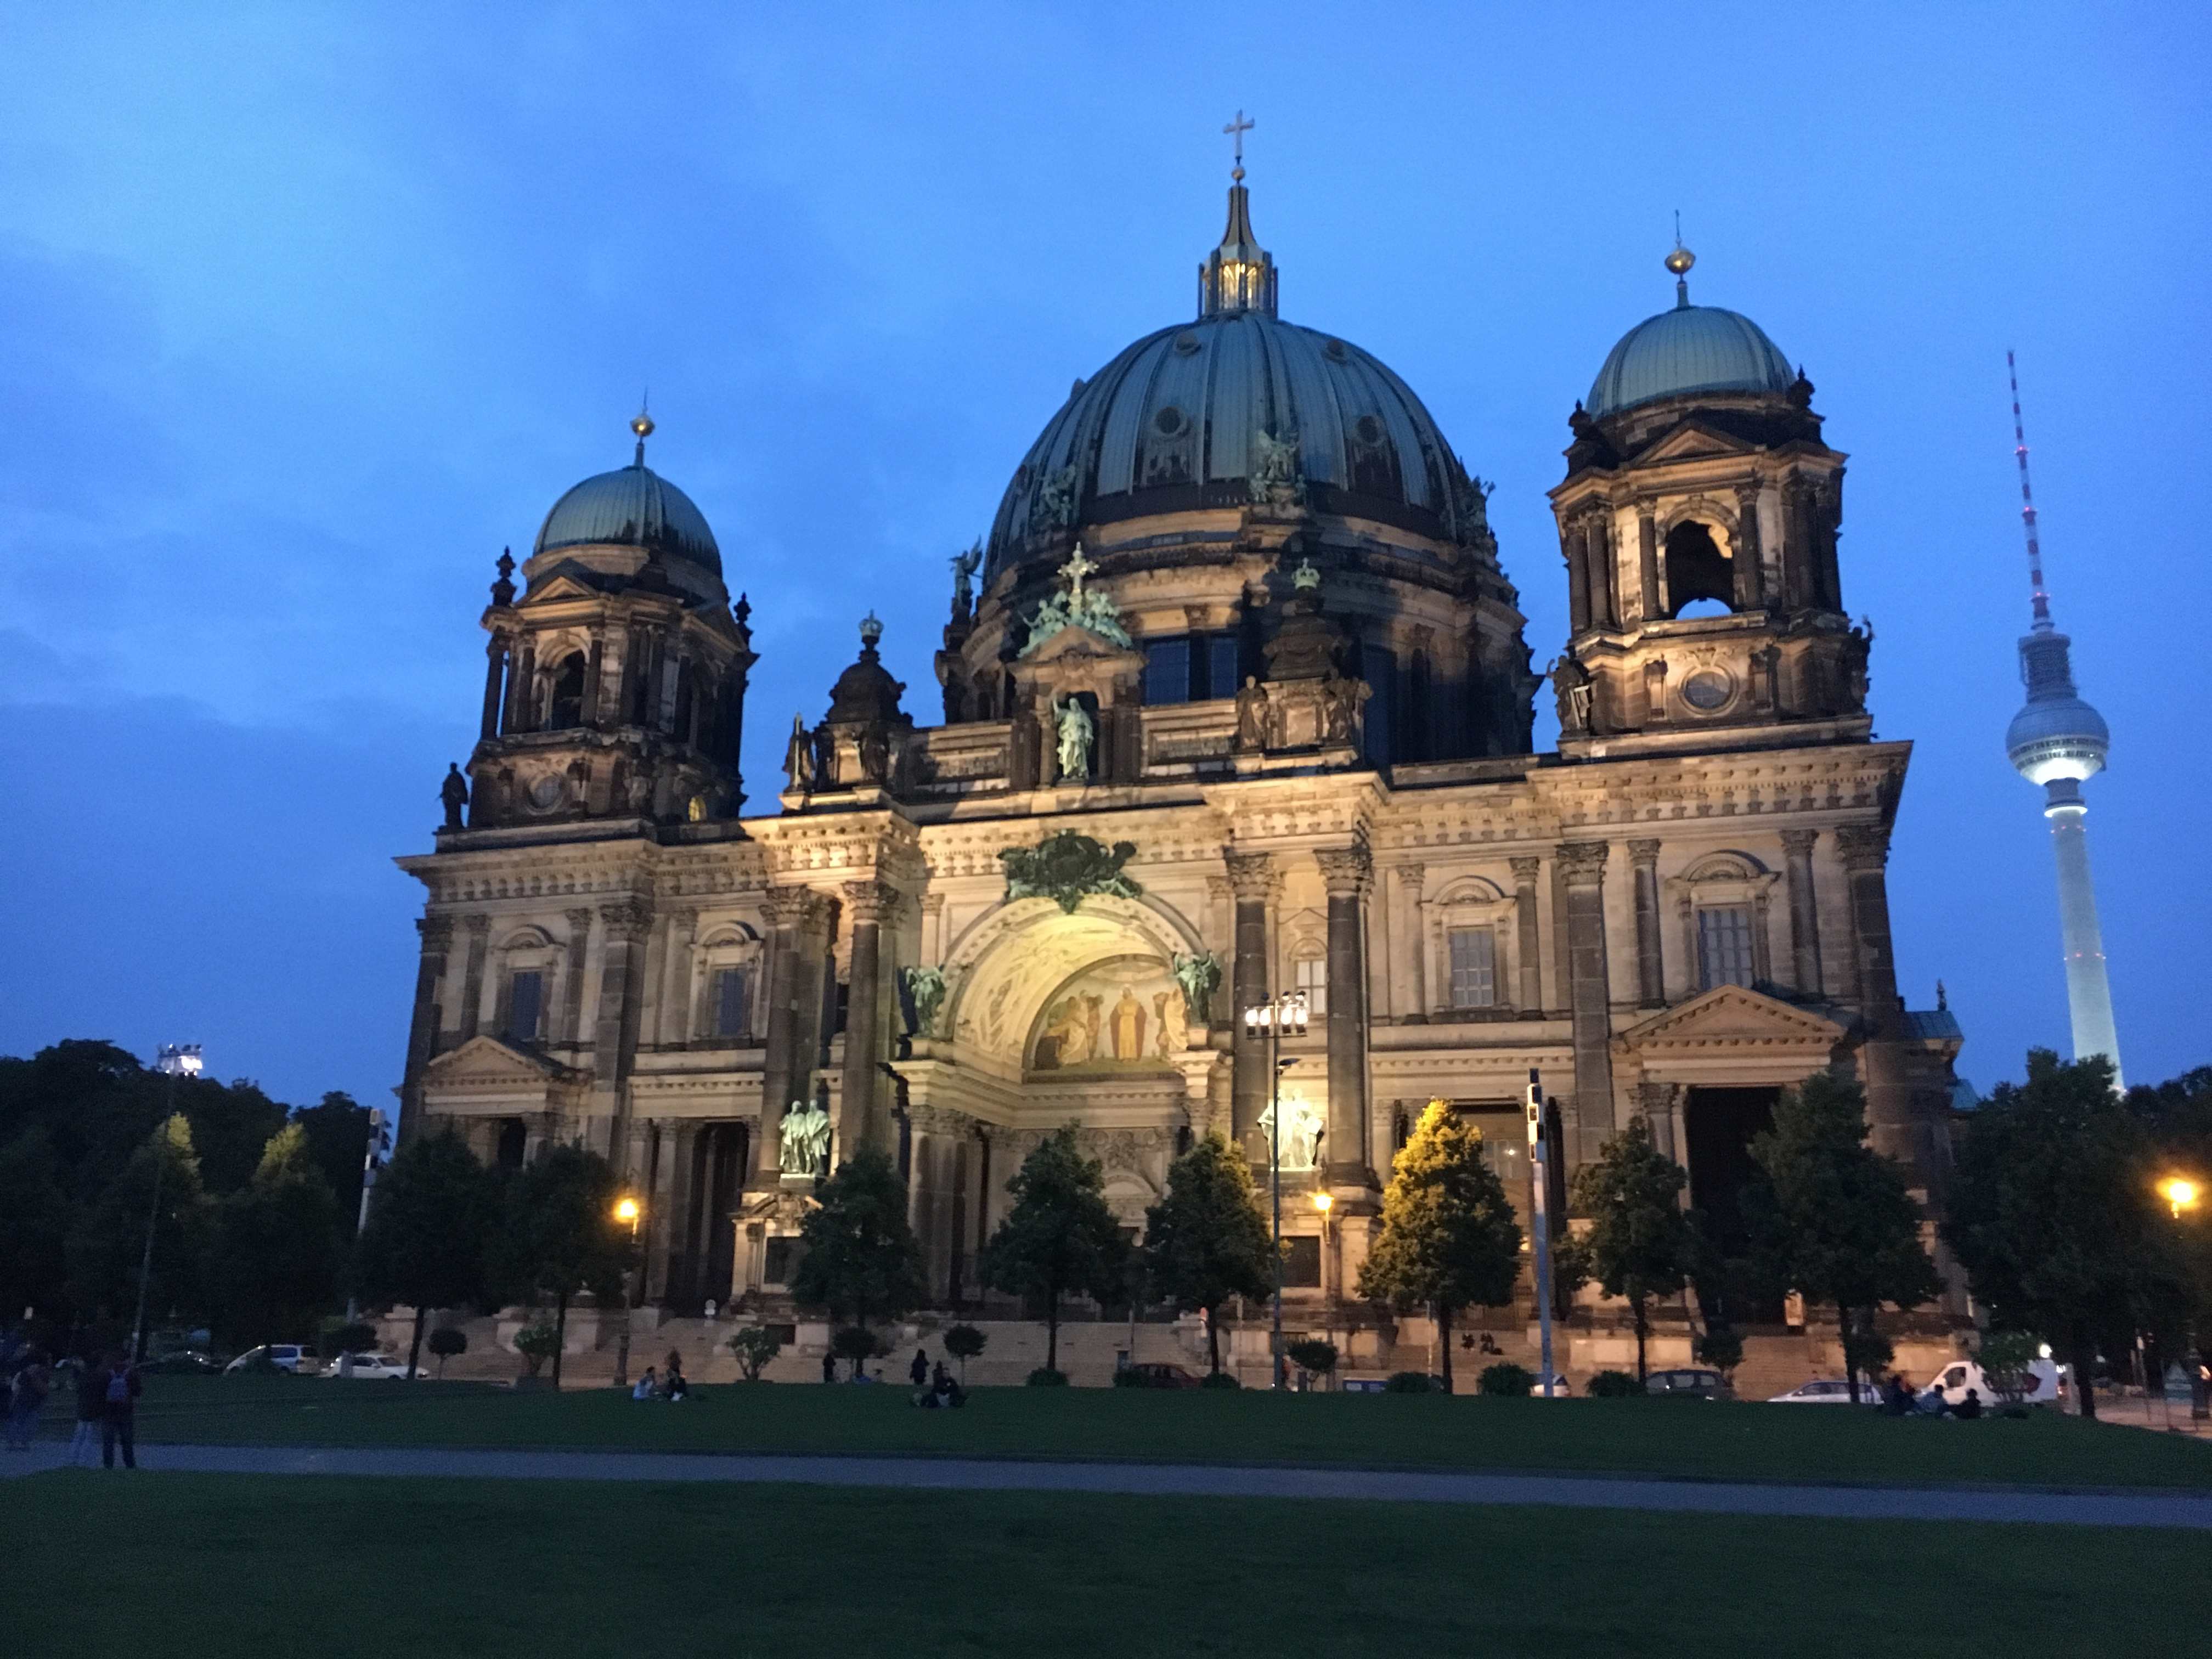
\includegraphics[width=\linewidth]{berlijn/berliner_dom.jpg}
    \caption{Berliner Dom}
  \end{subfigure}
  \begin{subfigure}[h]{0.48\textwidth}
    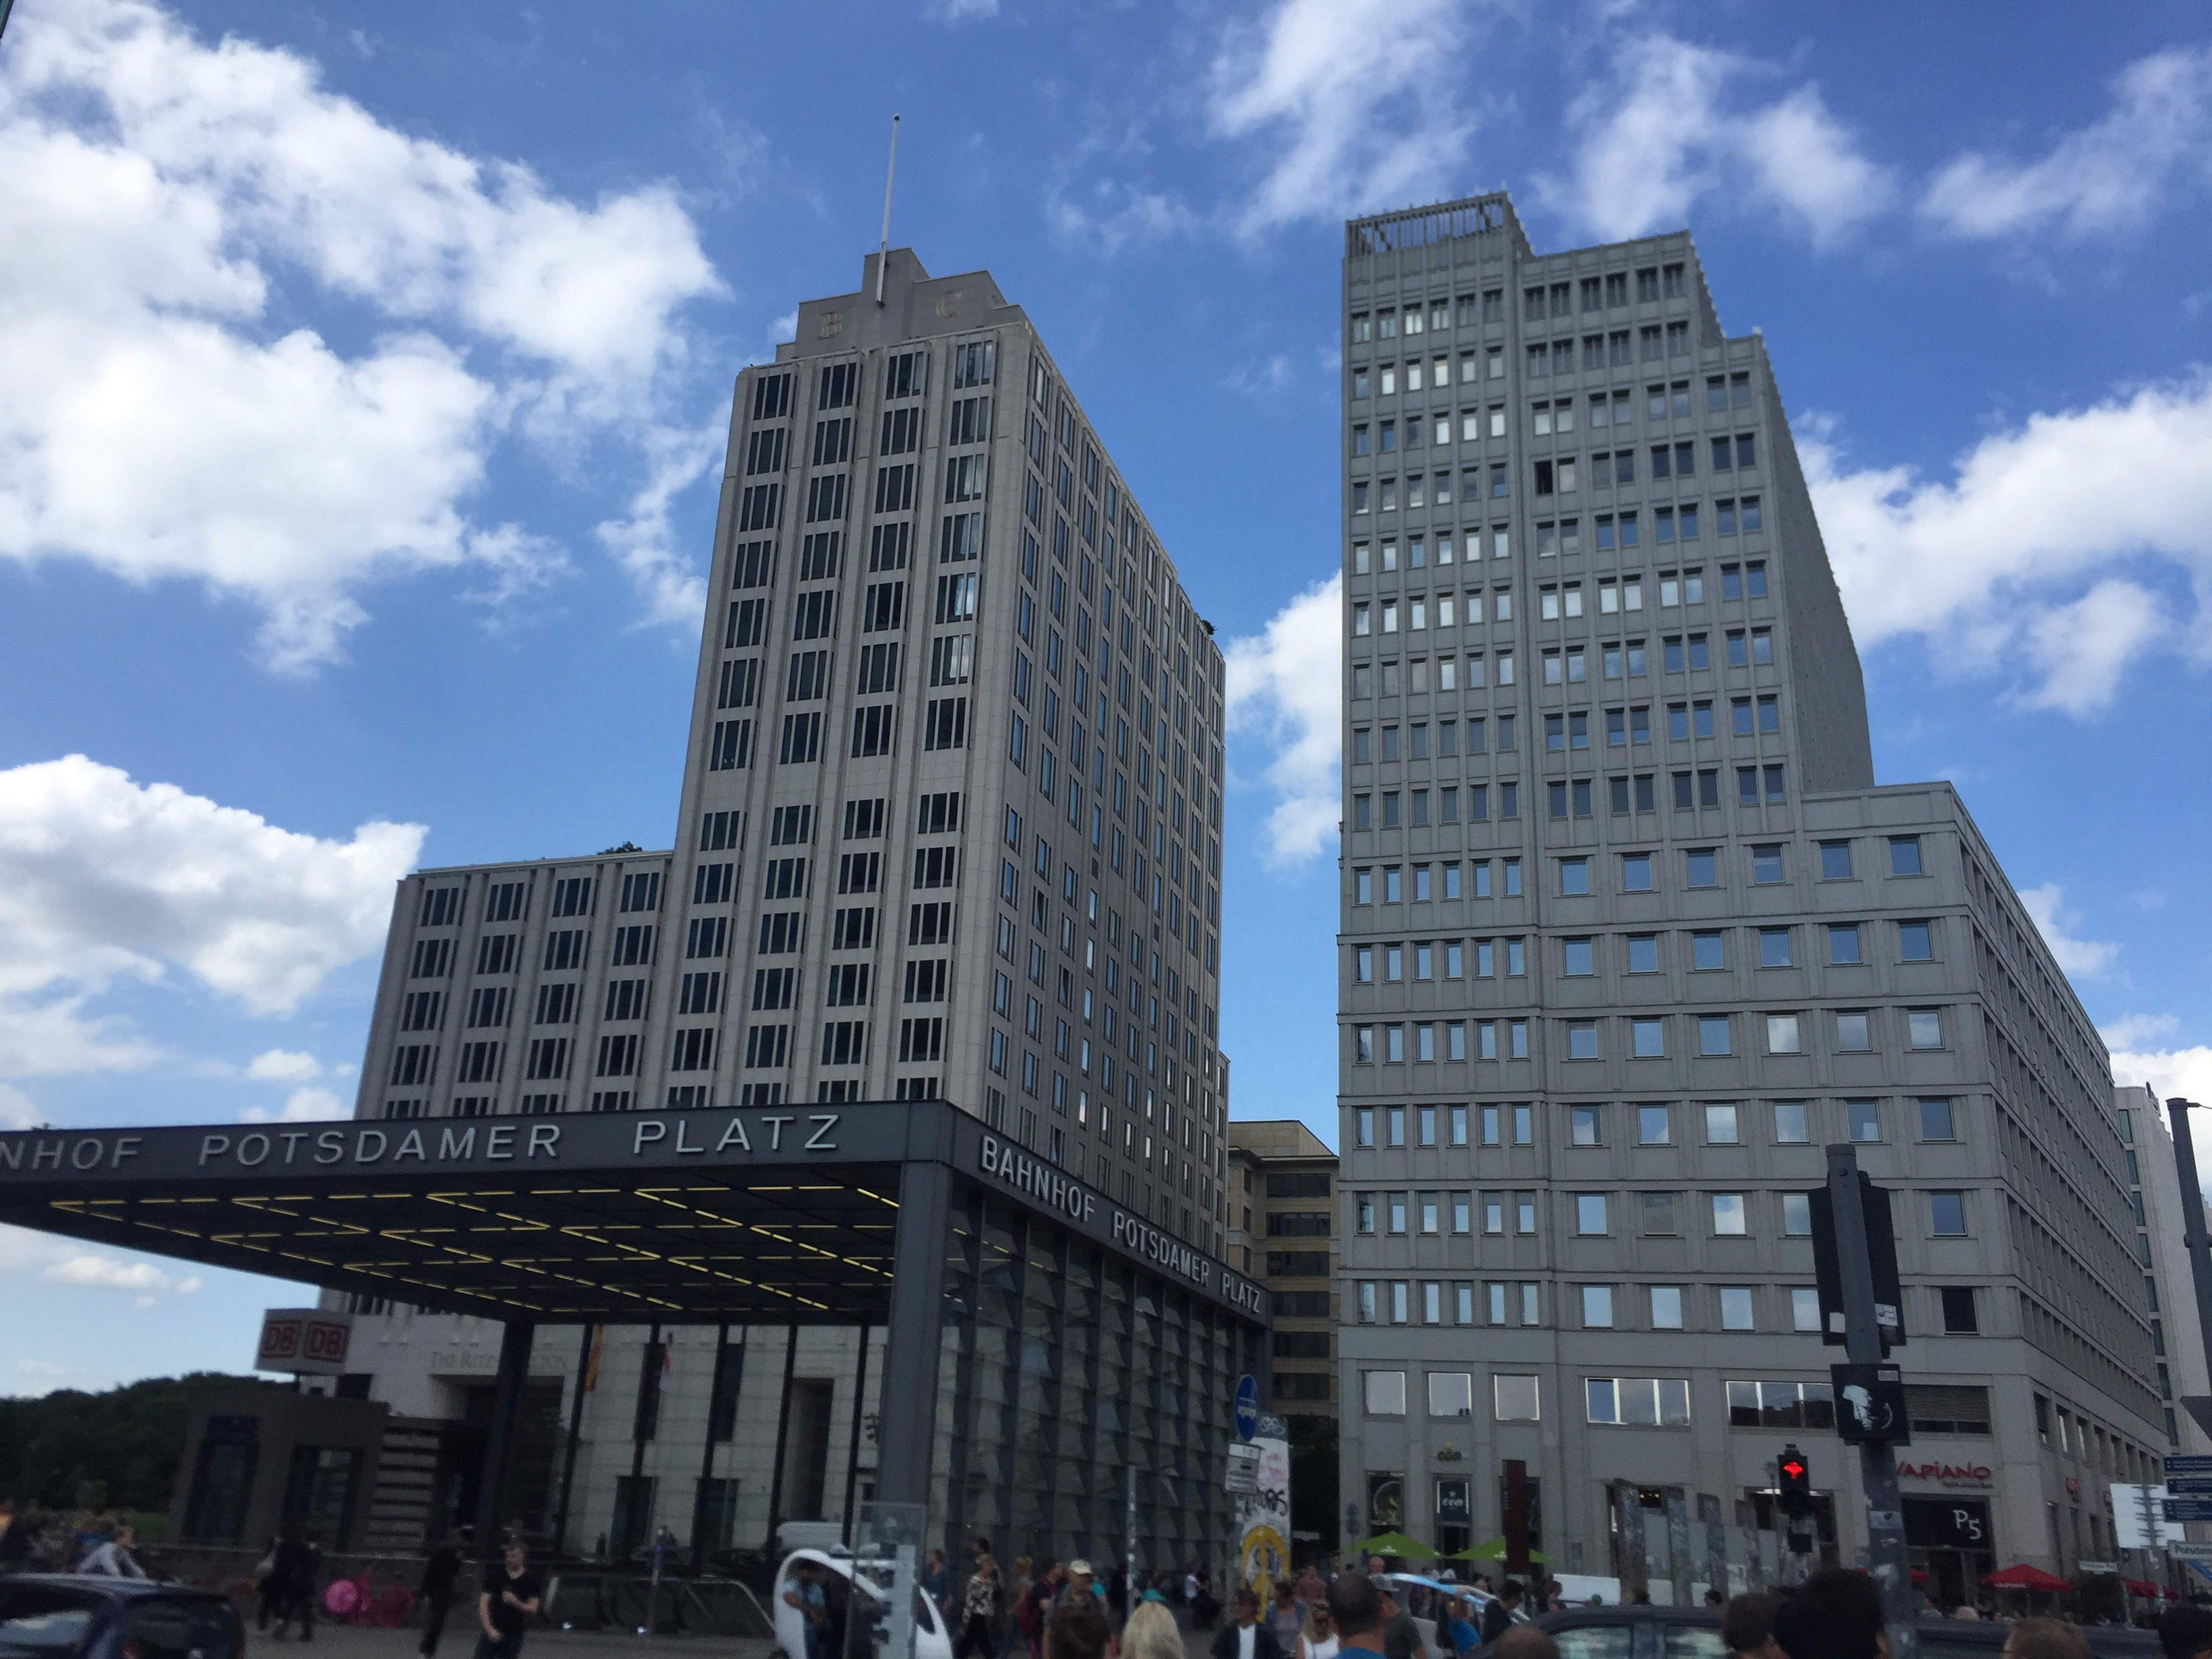
\includegraphics[width=\linewidth]{berlijn/potsdamer_platz.jpg}
    \caption{Portzdamer Platz}
  \end{subfigure}
  \begin{subfigure}[h]{0.48\textwidth}
    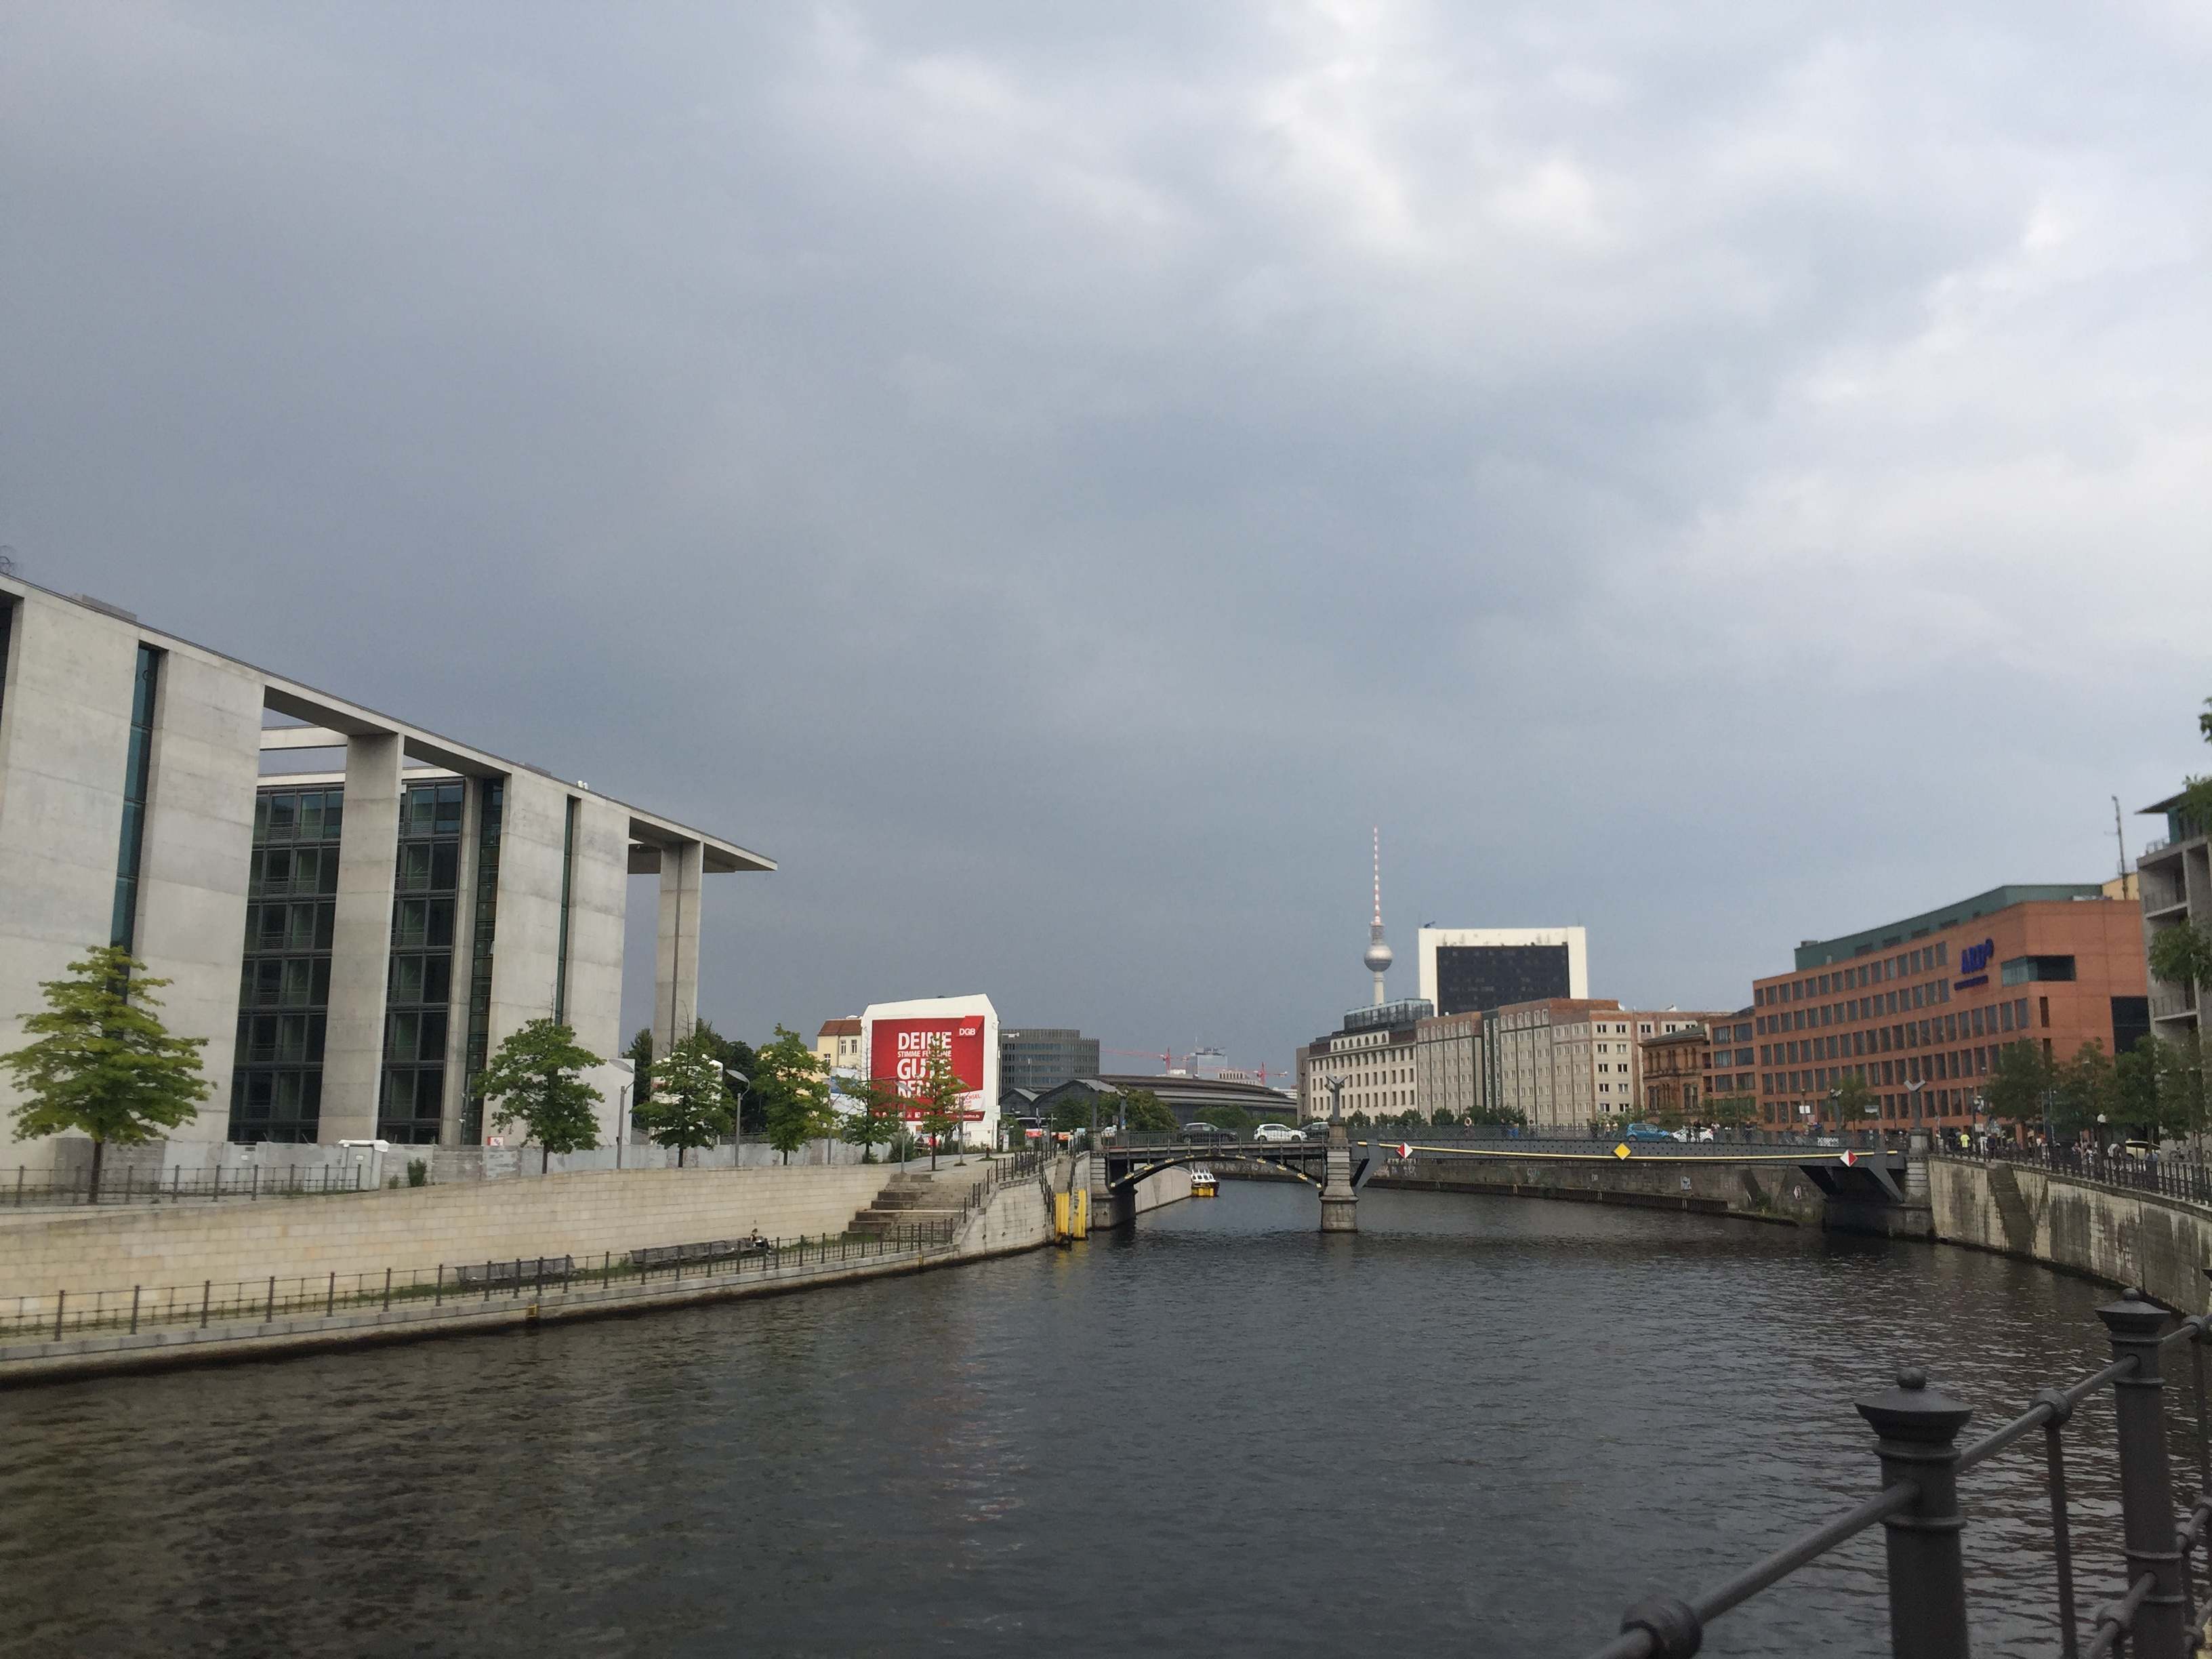
\includegraphics[width=\linewidth]{berlijn/uitzicht_reichstag.jpg}
    \caption{Uitzicht vanaf Reichstag}
  \end{subfigure}
  \begin{subfigure}[h]{0.48\textwidth}
    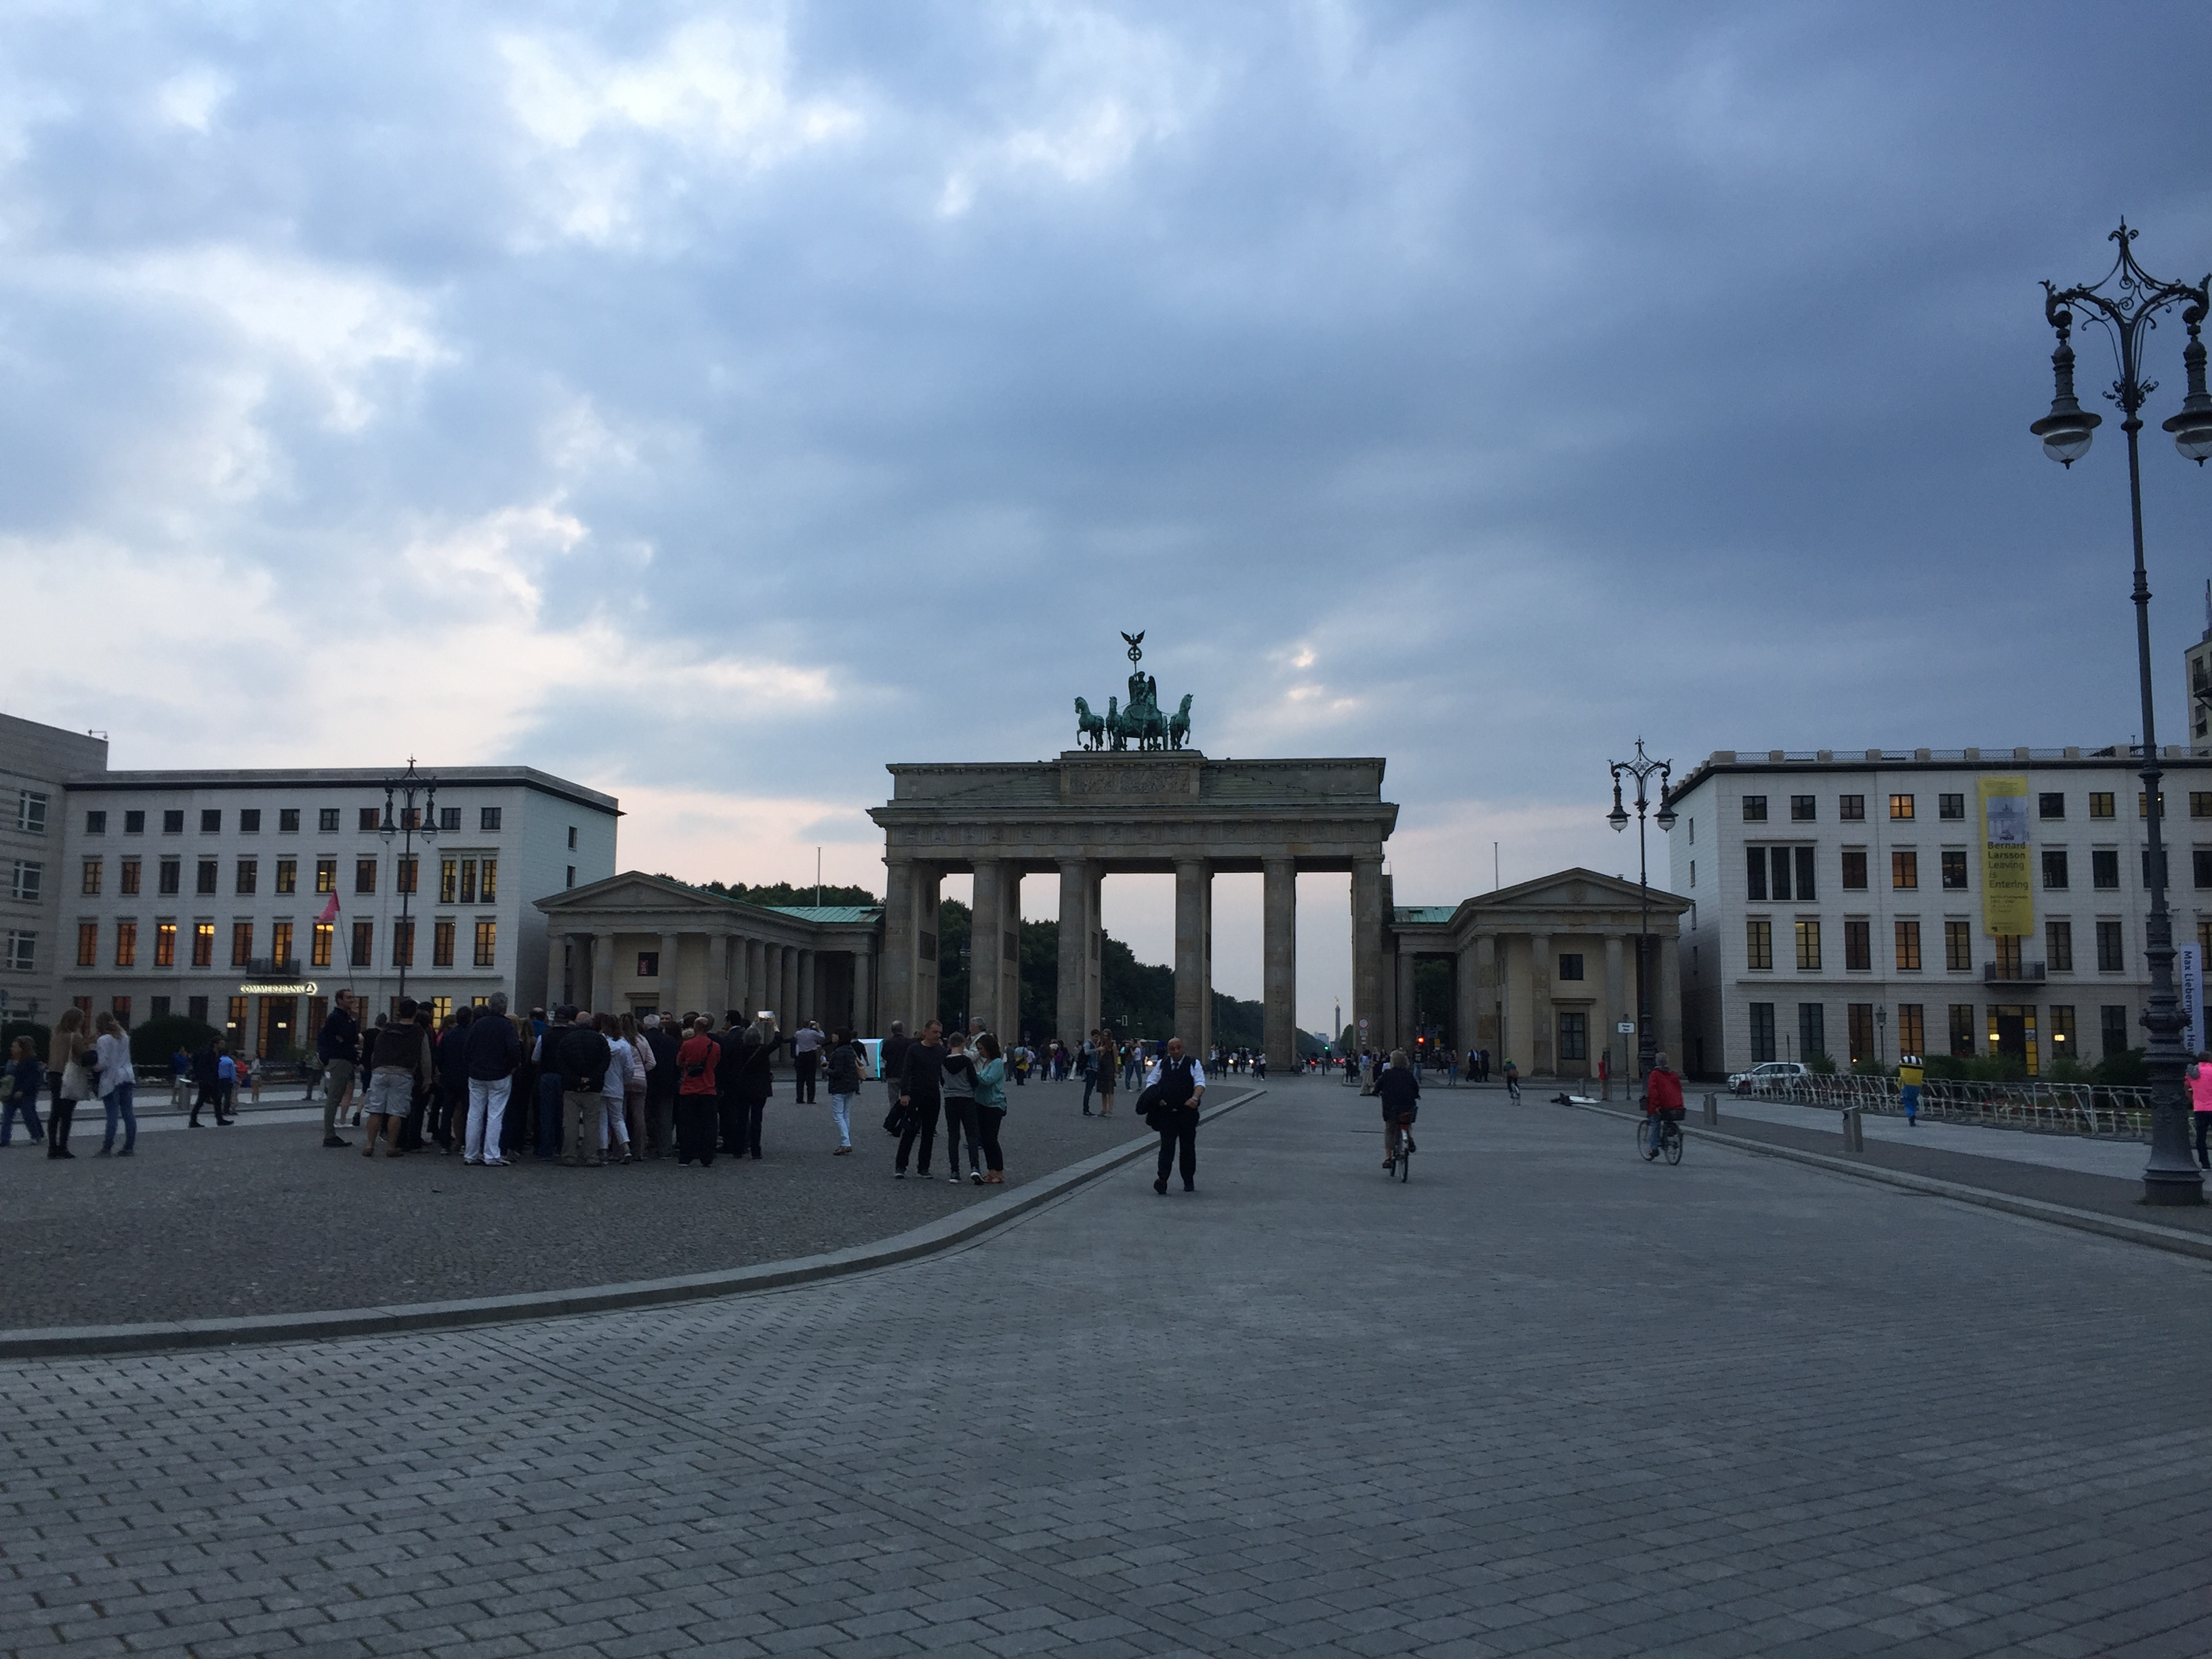
\includegraphics[width=\linewidth]{berlijn/brandenburger_tor.jpg}
    \caption{Brandenburger Tor}
  \end{subfigure}
\end{figure}